\documentclass[12pt]{article}
\usepackage{amsmath,amsthm,amssymb,amsfonts,fullpage,verbatim,bm,graphicx,enumerate,epstopdf,lscape,enumitem}
\usepackage[titletoc,title]{appendix}
\usepackage[dvipsnames,usenames]{color}
\usepackage[pdftex,pagebackref,colorlinks=true,pdfpagemode=UseNone,urlcolor=blue,linkcolor=blue,citecolor=BrickRed,pdfstartview=FitH,plainpages=true]{hyperref}
\usepackage[top=1.15in,bottom=1.15in,left=1.25in,right=1.25in,letterpaper]{geometry}
\usepackage[font=scriptsize]{caption}
\usepackage{cite}
\usepackage{caption,subcaption}



\begin{document}
\title{\textbf{Comparing different methods for predicting transcription factor binding from chromatin accessibility assays}}
\author{Zhengrong Xing}
\date{}
\maketitle


The analysis was done on the same dataset used in the msCentipede paper. DNase-seq and ChIP-seq data for a set of transcription factors (TFs) from the GM12878 LCL were used in the analysis. Two replicated DNase-seq measurements were available. A list of putative binding sites from the original analysis was provided for each of the TFs, together with the associated PWM scores for each site. Filtering of poorly mapped sites was also executed in an identical fashion (sites with $\leq80\%$ of uniquely mappable bases for a 64bp window around the motif were filtered out). The following 3 methods were then ran on each of the TFs, each of which will provide a ranking of the sites for each TF, with higher ranked sites more likely to be bound and vice versa:
\begin{enumerate}
\item Raw DNase counts, summed across a window of a specific length around the motif. More counts would result in a higher ranking.
\item CENTIPEDE. CENTIPEDE was run on all the sites, and the posterior probabilities from the software was used in the ranking, with higher probabilities implying higher rankings.
\item msCentipede. msCentipede was run on sites with PWM score $\geq13$ to fit the model, and the learned model was then run on all the sites to provide posterior probabilities. Higher probabilities translate to higher rankings.
\end{enumerate}

For each of the above methods, different window sizes around the motif were used to determine the effect of the window size on the performance of the methods. Specifically, windows of $2^6,2^7,2^8,2^9,2^{10}$bp were used in the analysis.

Evaluation of the performance of the methods was done through ROC curves, area under ROC (auROC) in particular. The gold standard was generated based on the ChIP-seq experiment, with bound sites being ones that lay entirely within a ChIP-seq peak as defined by MACS (at 1\% FDR cutoff). Unbound sites were defined slightly differently than the original analysis (due to unfamiliarity with the control experiment used in the original analysis), so that unbound sites were ones which did not fall entirely within ChIP-seq peaks, and also had total ChIP-seq reads less than the median across all the sites for the corresponding TF.

The plots below show some representative plots of auROC values across different window sizes for each TF, sorted by their relative frequency of occurrence. For most of the TFs, the first plot illustrates what happens. Dcuts (for DNase cuts) performs consistently better than msCentipede and CENTIPEDE (to varying degrees based on the TF in question), and the auROC peaks at a window size larger than what was used in the original analysis, which was 64bp. The peak for Dcuts can happen at 256, 512 or 1024bp. 
\begin{center}
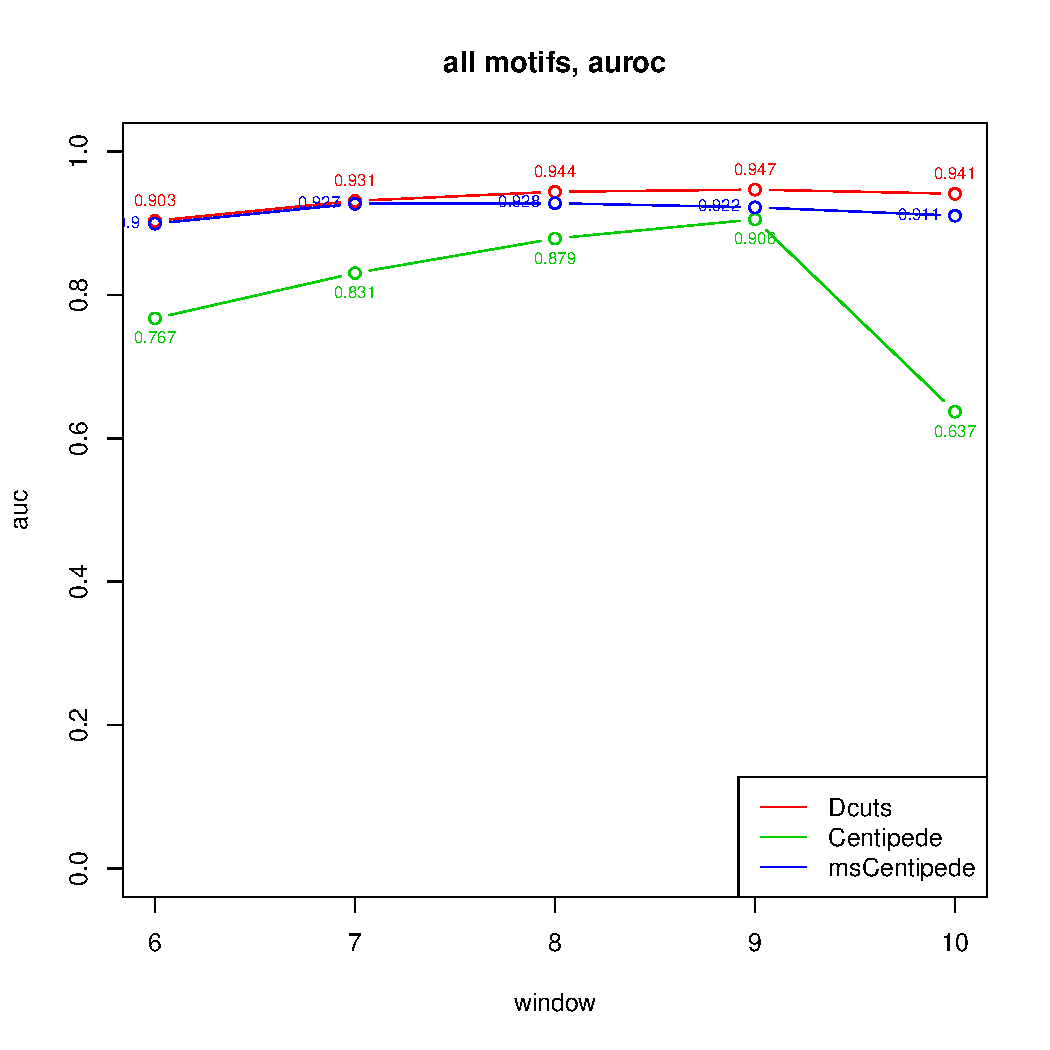
\includegraphics[width=0.5\textwidth]{1_dcuts_better_and_plateaus.pdf}
\end{center}

The next plot shows perfect auROC for all the window sizes and is not of interest, but occurs frequently.
\begin{center}
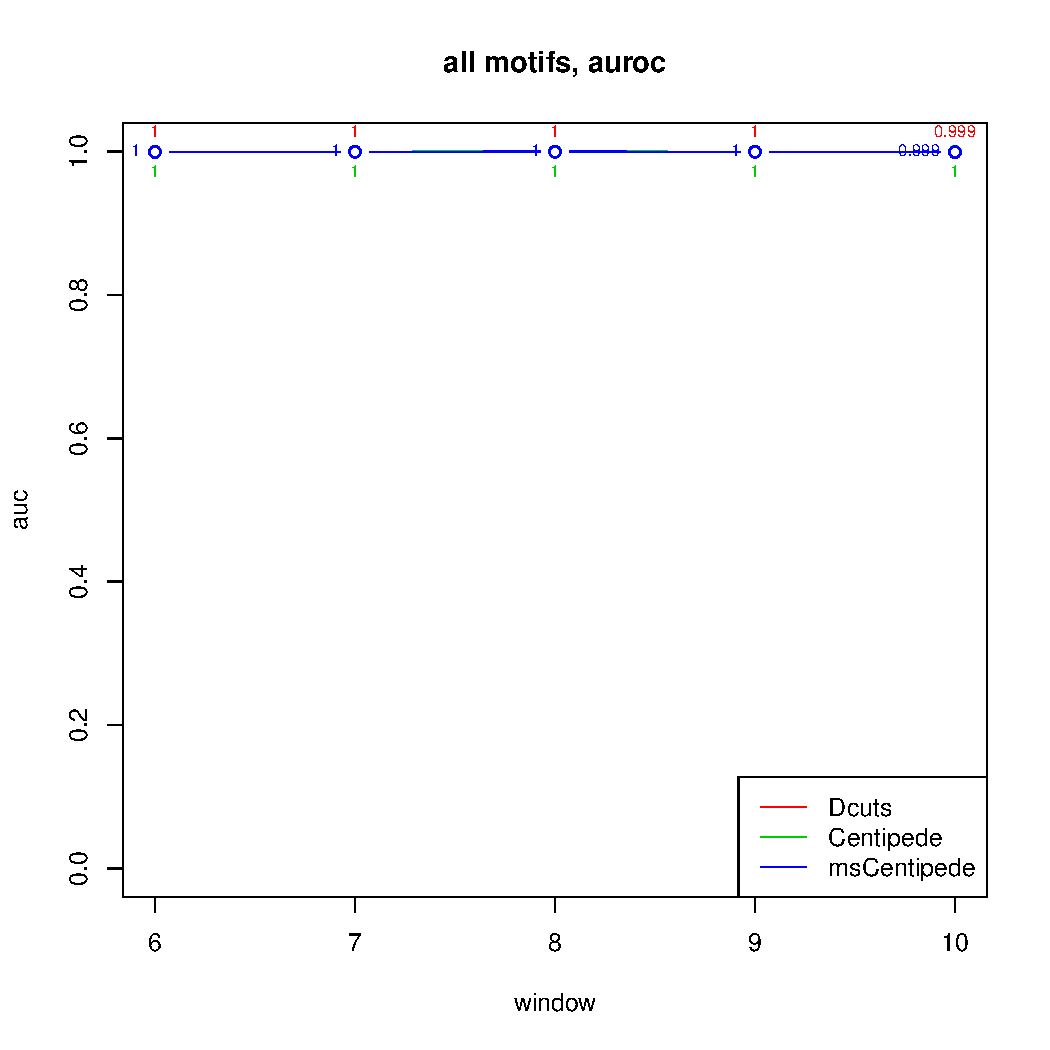
\includegraphics[width=0.5\textwidth]{2_perfect_auc.pdf}
\end{center}

The third plot shows shows that Dcuts performs worse than msCentipede (but typically better than CENTIPEDE) for small window sizes, but better for larger ones. Overall Dcuts still outperforms msCentipede by taking the max auROC across all window sizes.
\begin{center}
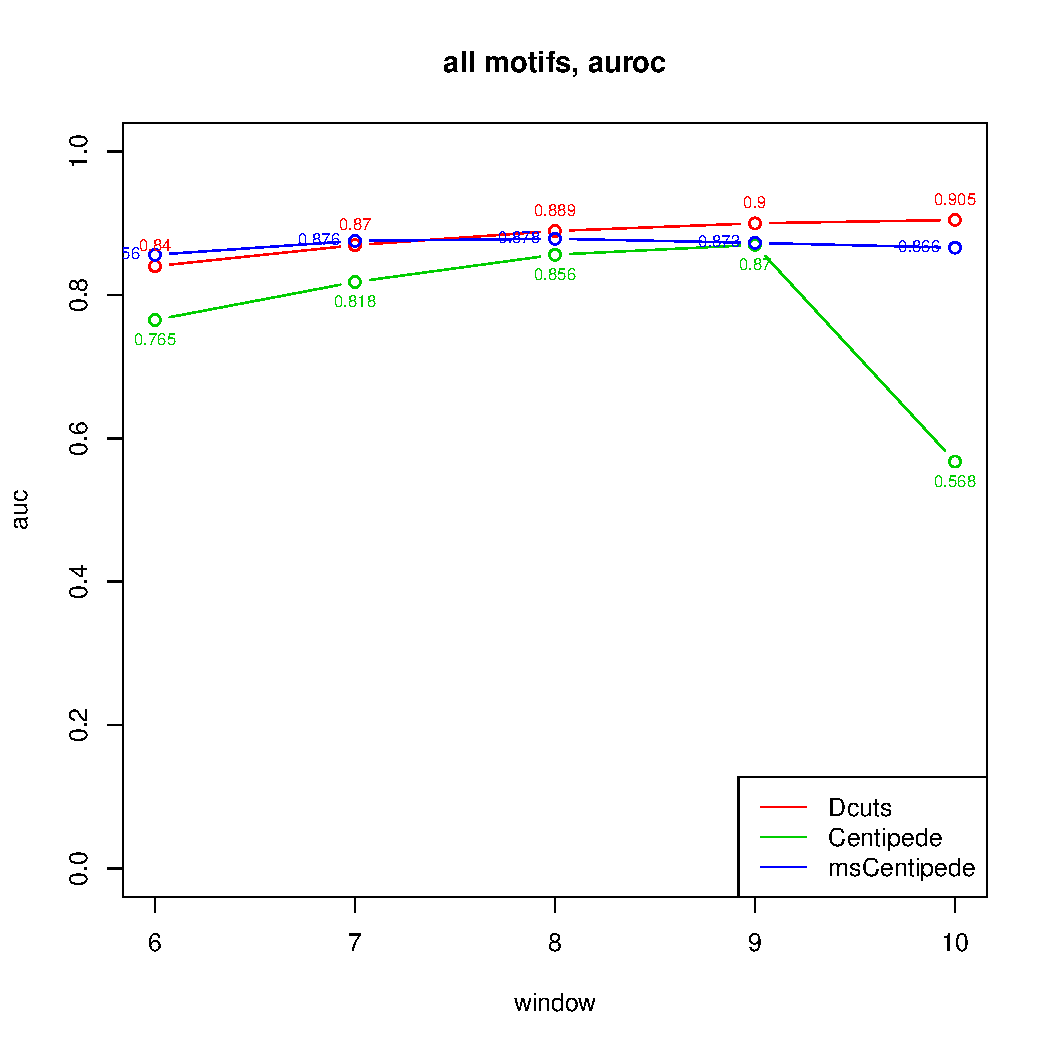
\includegraphics[width=0.5\textwidth]{3_dcuts_mscent_cross.pdf}
\end{center}

The next plot shows that Dcuts and msCentipede are virtually identical, but both outperform CENTIPEDE.
\begin{center}
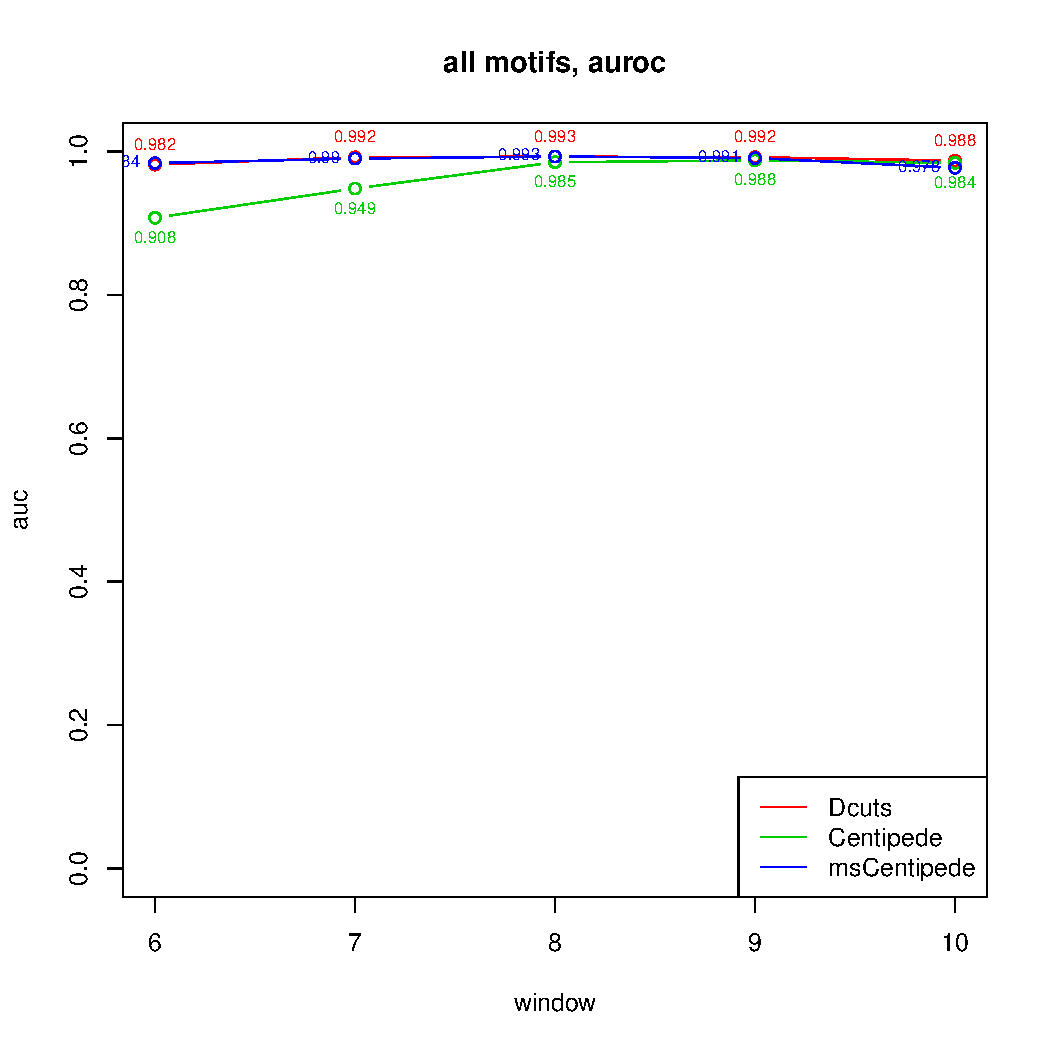
\includegraphics[width=0.5\textwidth]{4_dcuts_mscent_same.pdf}
\end{center}

The fifth plot shows that msCentipede outperforms Dcuts by a lot for small window sizes (and underperforms only by a little for later window sizes), and overall outperforms Dcuts. This only happens in MAFK, which appears to have a weaker relationship between chromatin accessibility (DNase-seq) and binding affinity (ChIP-seq) compared to the other TFs (low auROCs for all the methods).
\begin{center}
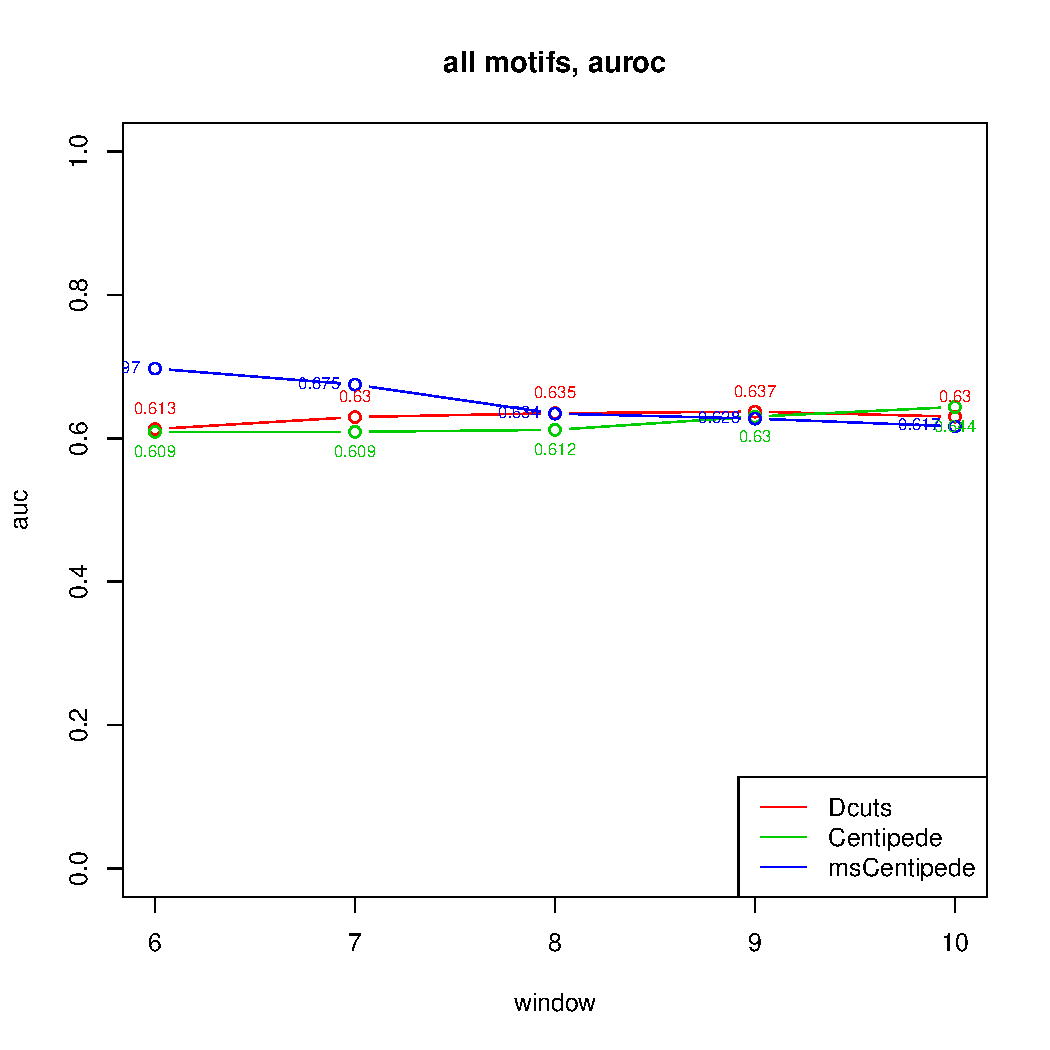
\includegraphics[width=0.5\textwidth]{5_mscent_better_small.pdf}
\end{center}

The final plot shows that msCentipede outperforms Dcuts for all window sizes. This only happens in CTCF.
\begin{center}
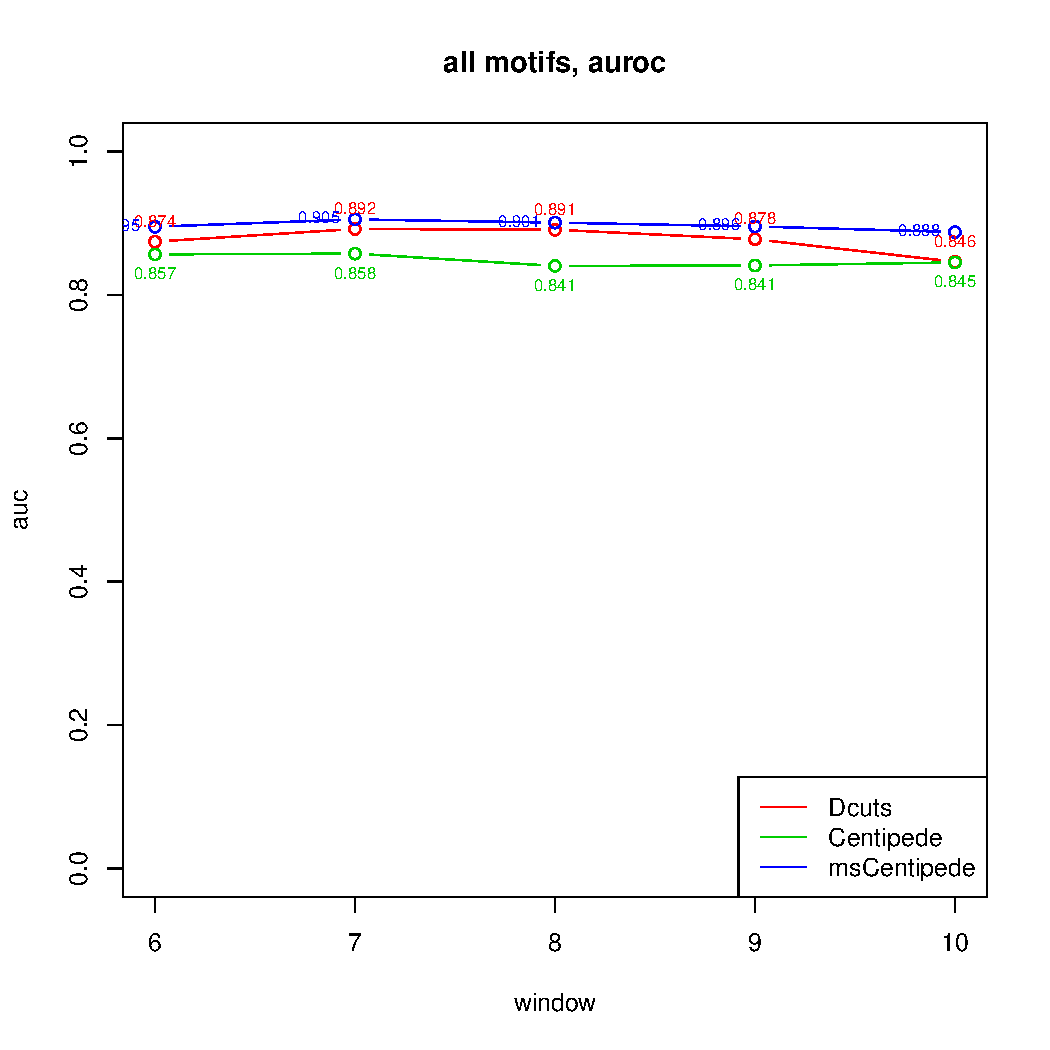
\includegraphics[width=0.5\textwidth]{6_mscent_better.pdf}
\end{center}

Overall, it seems that using raw DNase cuts is generally better than using msCentipede or CENTIPEDE, especially if we consider larger windows around the motif sites (although there typically is a certain window size after which performance will start to drop, which could be 256, 512 or 1024bp). Furthermore, from supervised learning done using Multiseq it appears that the total number of DNase cuts contributes a lot more to binding compared to the actual DNase profile. Direct comparison of the ranking from the methods against the actual ChIP-seq reads further supports these facts, as Dcuts tend to have higher rank correlations with ChIP-seq reads than either msCentipede or CENTIPEDE.
\end{document}